\documentclass[a4paper,11pt]{article}

\usepackage[T1]{fontenc}
\usepackage[margin=1in]{geometry}
\usepackage{graphicx}
\usepackage{capt-of}

\graphicspath{{./}}
\renewcommand{\thefigure}{S\arabic{figure}}

\title{Supplementary Material\\An Interpretable Statistical Surrogate of Activated Sludge Systems that Preserves Mass Conservation and Component Non-Negativity}
\author{}
\date{}

\begin{document}

\maketitle

\section*{Target-Wise Interpretability Atlases}

This supplementary file collects the complete target-wise ICSOR raw-head interpretability atlases that are not retained in the main manuscript. Figure~4 of the manuscript is reserved for the COD raw-head $\Theta_{cc}$ block only, so the paper can discuss one representative interaction surface without repeating four dense multi-block panels in the main text. Figures~\ref{fig:supp_cod_interpretability}--\ref{fig:supp_tss_interpretability} provide the full COD, TN, TP, and TSS raw-head atlases.

Each atlas presents the reported-target coefficient blocks obtained from the pre-correction raw-head map $I_{comp}(I_F-\Gamma)^{-1}B$: the scalar bias term $b$, the first-order operational block $W_u$, the first-order influent block $W_{in}$, the operational-curvature block $\Theta_{uu}$, and the operation--influent and influent-curvature blocks $\Theta_{uc}$ and $\Theta_{cc}$. The component-space coupling matrix $\Gamma$ is also shown as a shared structural panel. The ASM component basis is kept complete in every applicable panel, and the heatmaps are drawn from the lower origin so the operational axes begin at HRT and then Aeration. These atlases describe the globally defined raw regression head; the final affine/LP deployment map is piecewise and therefore does not have one global coefficient atlas.

\begin{figure}[p]
\centering
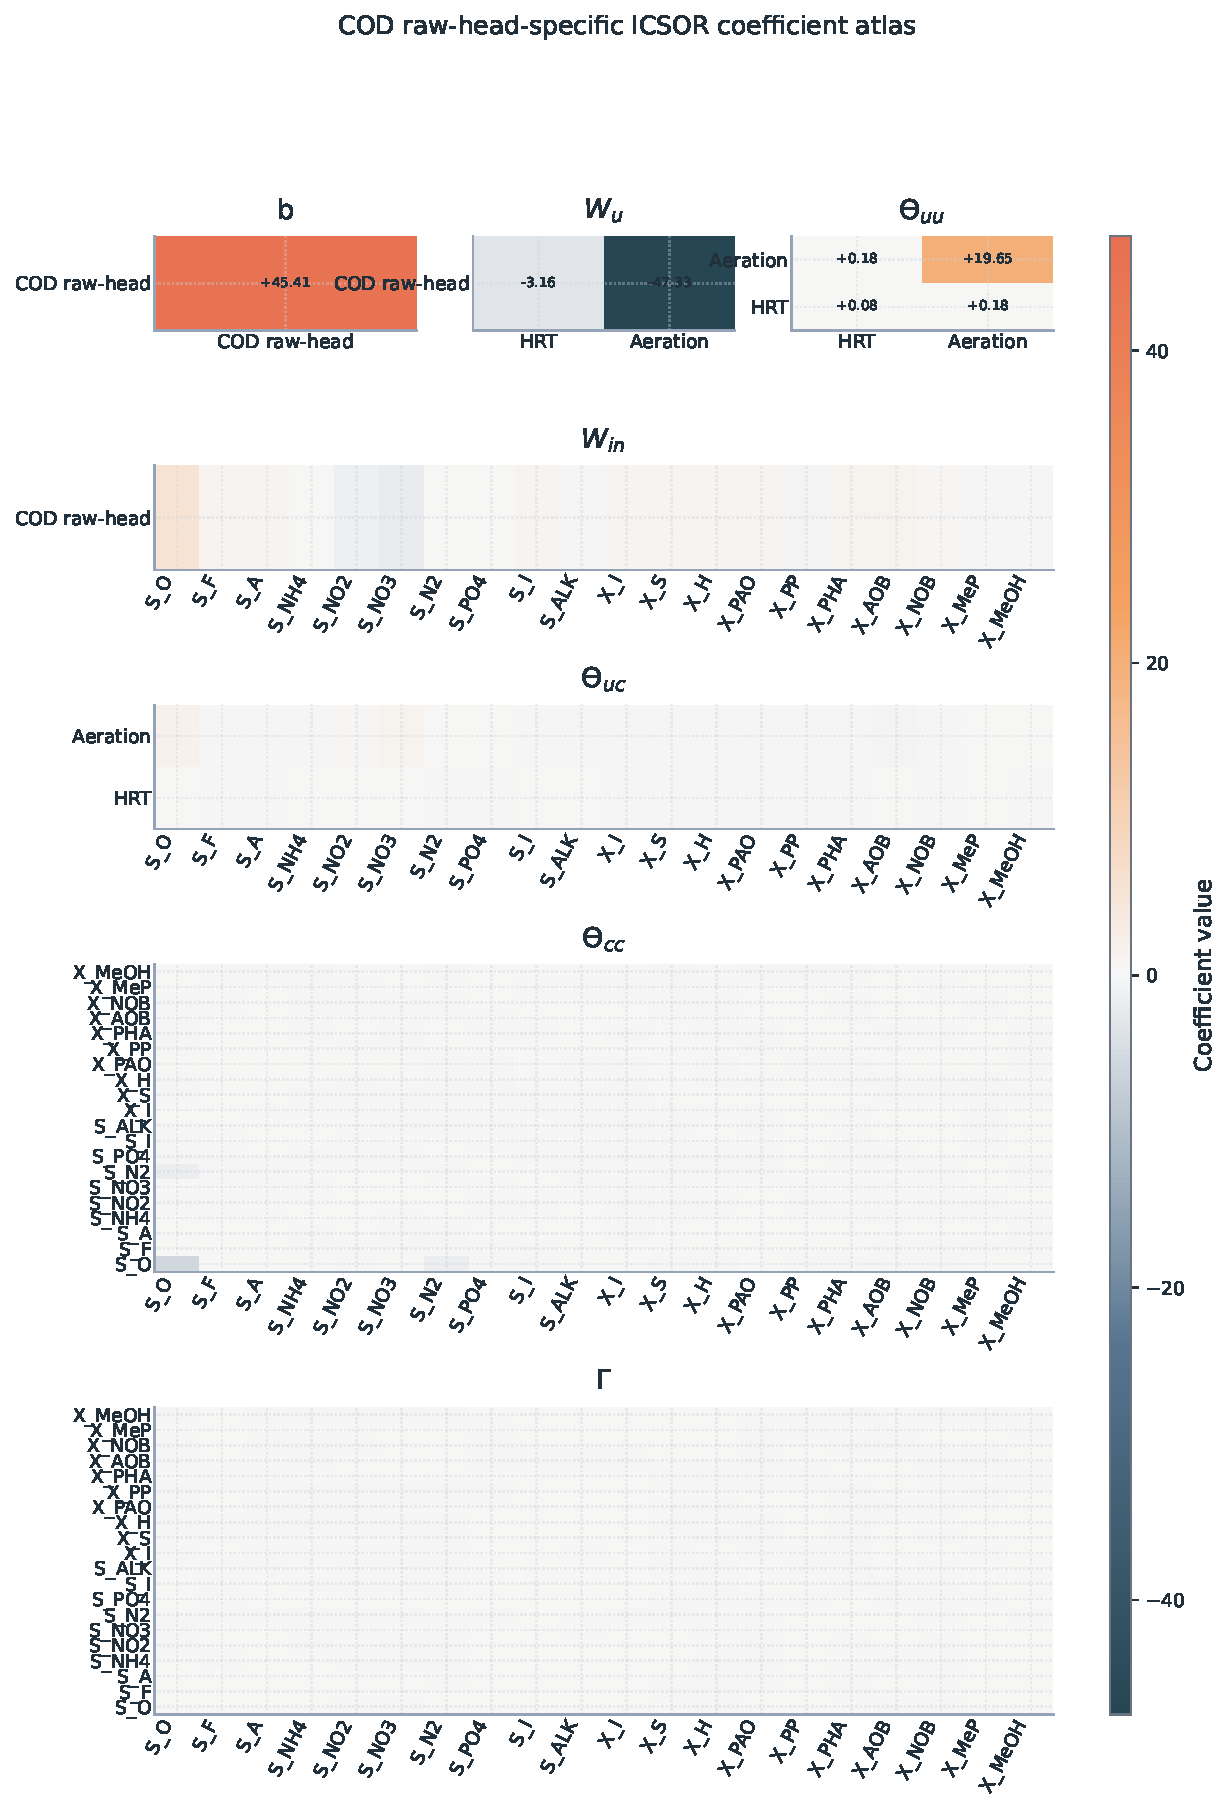
\includegraphics[width=\textwidth,height=0.90\textheight,keepaspectratio]{figureS1_cod_icsor_structure.pdf}
\caption{COD raw-head ICSOR coefficient atlas showing the reported-target blocks of $I_{comp}(I_F-\Gamma)^{-1}B$ together with the shared component-space coupling matrix $\Gamma$. The symmetric $\Theta_{uu}$ and $\Theta_{cc}$ panels display mirrored off-diagonal cells.}
\label{fig:supp_cod_interpretability}
\end{figure}

\begin{figure}[p]
\centering
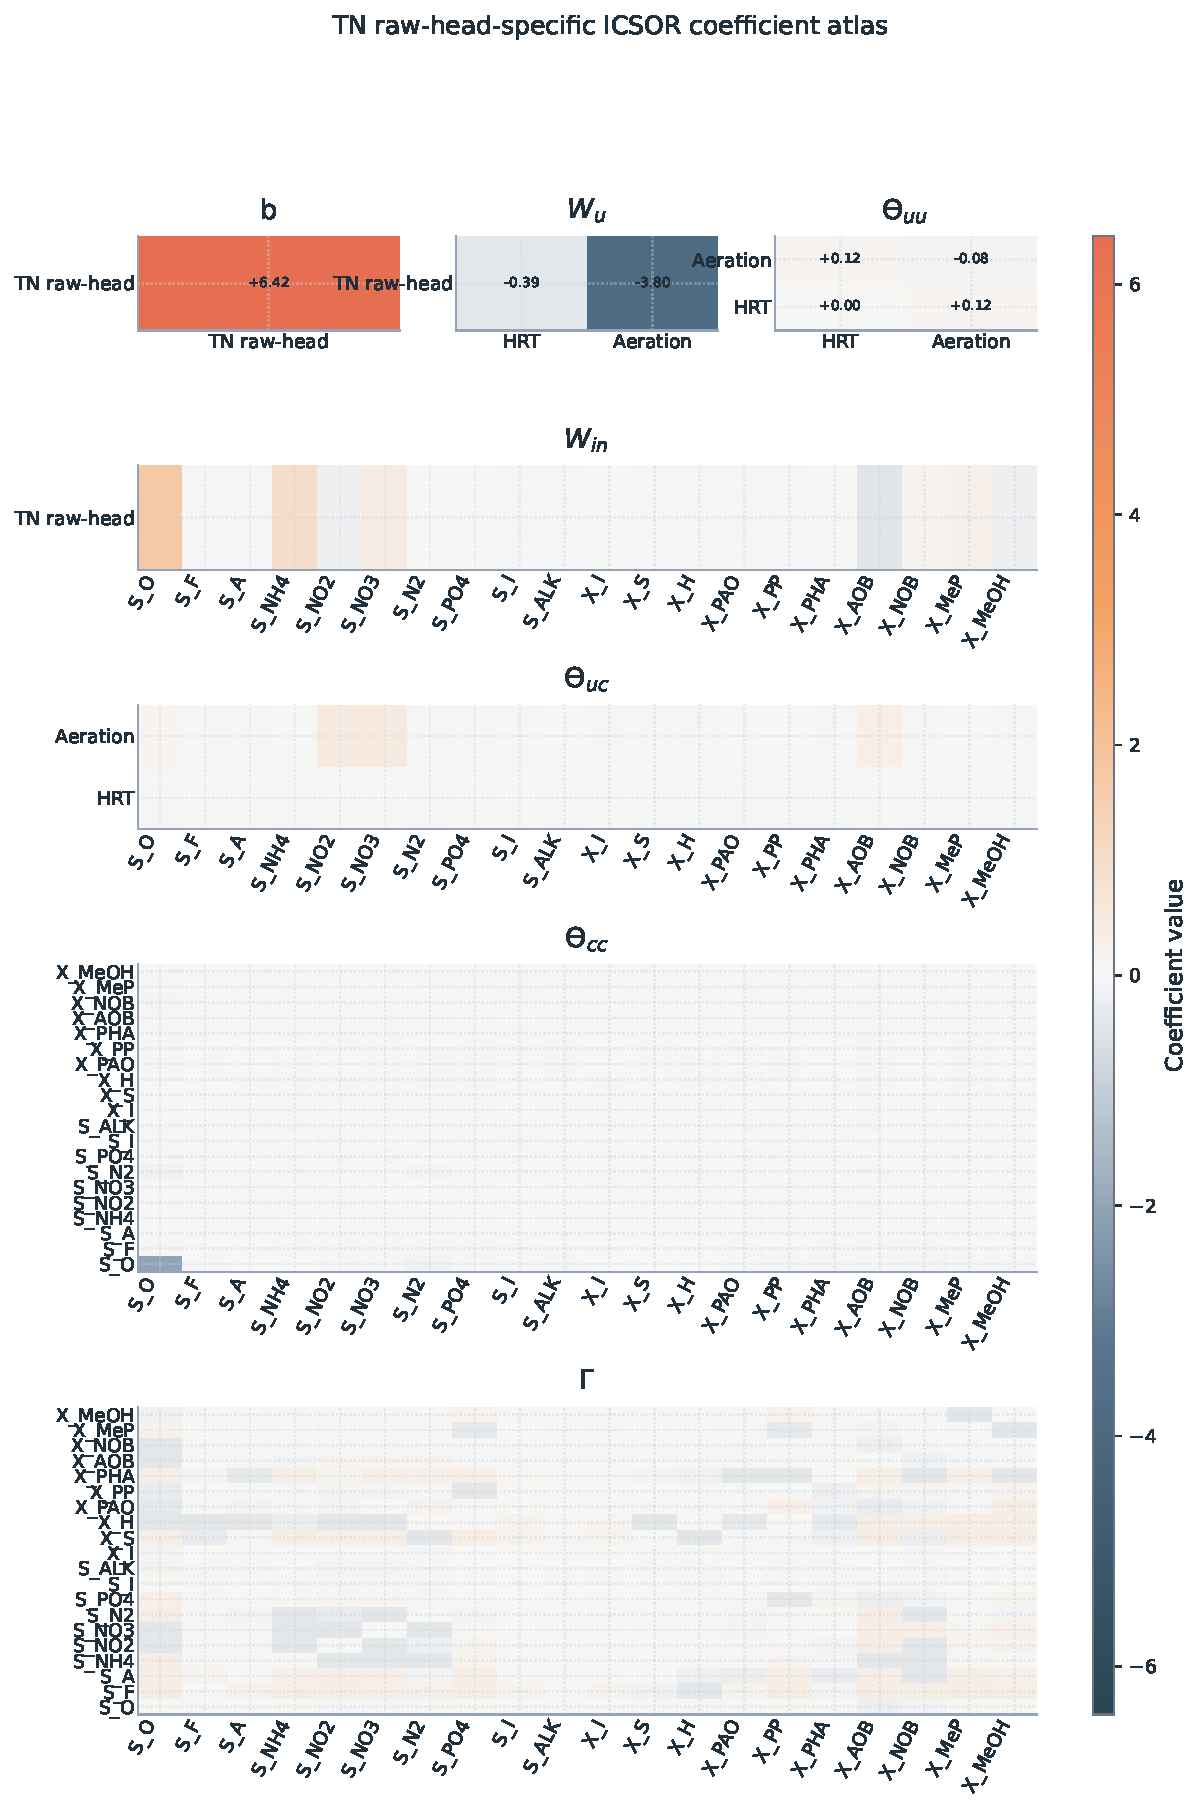
\includegraphics[width=\textwidth,height=0.90\textheight,keepaspectratio]{figureS2_tn_icsor_structure.pdf}
\caption{TN raw-head ICSOR coefficient atlas showing the reported-target blocks of $I_{comp}(I_F-\Gamma)^{-1}B$ together with the shared component-space coupling matrix $\Gamma$. The symmetric $\Theta_{uu}$ and $\Theta_{cc}$ panels display mirrored off-diagonal cells.}
\label{fig:supp_tn_interpretability}
\end{figure}

\begin{figure}[p]
\centering
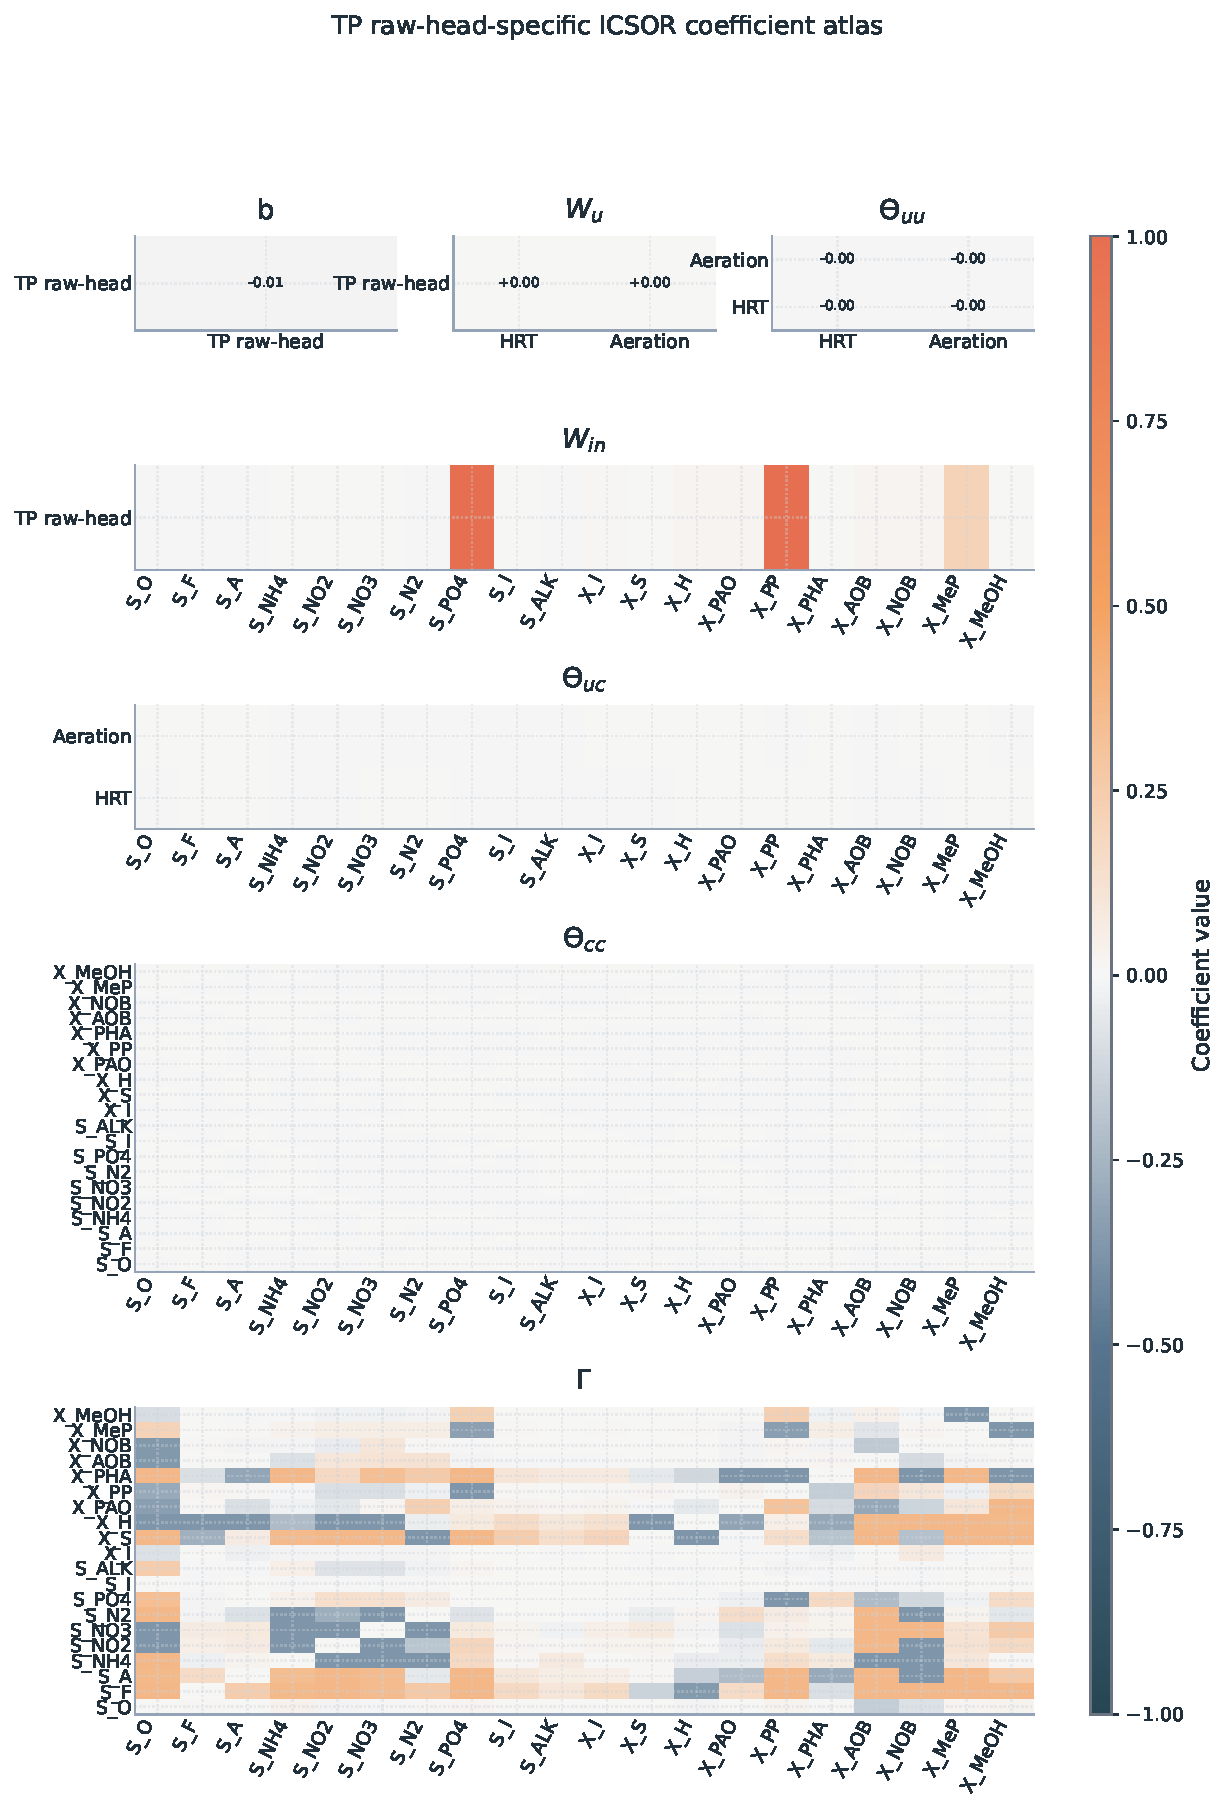
\includegraphics[width=\textwidth,height=0.90\textheight,keepaspectratio]{figureS3_tp_icsor_structure.pdf}
\caption{TP raw-head ICSOR coefficient atlas showing the reported-target blocks of $I_{comp}(I_F-\Gamma)^{-1}B$ together with the shared component-space coupling matrix $\Gamma$. The symmetric $\Theta_{uu}$ and $\Theta_{cc}$ panels display mirrored off-diagonal cells.}
\label{fig:supp_tp_interpretability}
\end{figure}

\begin{figure}[p]
\centering
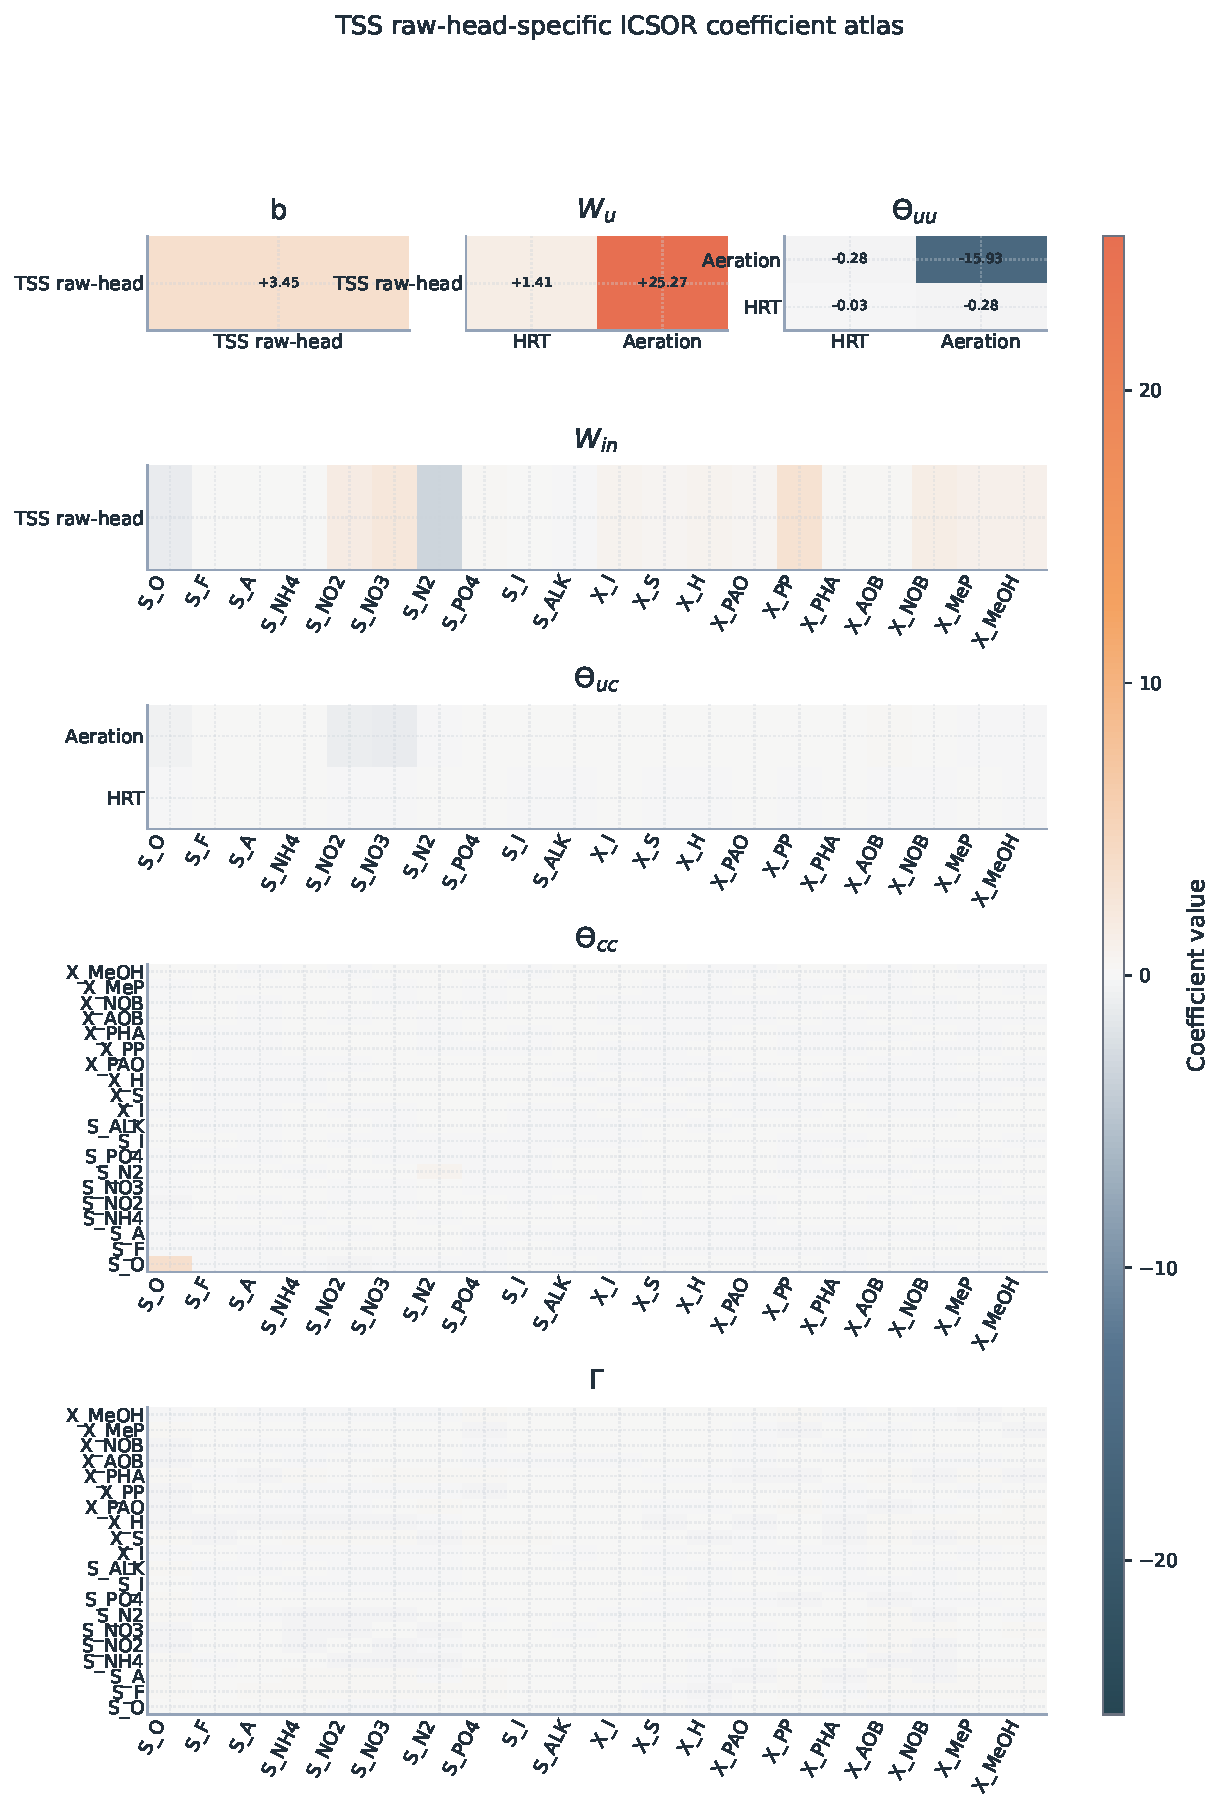
\includegraphics[width=\textwidth,height=0.90\textheight,keepaspectratio]{figureS4_tss_icsor_structure.pdf}
\caption{TSS raw-head ICSOR coefficient atlas showing the reported-target blocks of $I_{comp}(I_F-\Gamma)^{-1}B$ together with the shared component-space coupling matrix $\Gamma$. The symmetric $\Theta_{uu}$ and $\Theta_{cc}$ panels display mirrored off-diagonal cells.}
\label{fig:supp_tss_interpretability}
\end{figure}

\end{document}
